\chapter{Repetition - \keyword{For}, \keyword{While} and \keyword{Do}}
\label{ch:repetition}

This chapter explains:
  \begin{itemize}
    \item how to perform repetitions (loops) using \keyword{For} statements;
    \item how to perform repetitions using \keyword{While} statements;
    \item how to perform repetitions using \keyword{Do} statements;
    \item how to choose which kind of loop to use;
    \item how to use \keyword{And}, \keyword{Or} and \keyword{Not} in loops;
    \item how to combine repetitions with selections.
  \end{itemize}

  \section{Introduction}
		We humans are used to doing things again and again - eating, sleeping and working. Computers similarly routinely perform repetition. Examples are:
		\begin{itemize}
	    \item adding up a list of numbers;
  	  \item searching files for some desired information;
    	\item solving a mathematical equation iteratively, by repeatedly obtaining better and better approximations;
	    \item making a graphical image move on the screen (animation).
		\end{itemize}
		We have already seen that a computer obeys a \emph{sequence} of instructions. Now we shall see how to repeat a sequence of instructions a number of times. Part of the power of computers arises from their ability to perform repetitions extremely quickly. In the language of programming, a repetition is called a \emph{loop}.
		
		There are three ways in which the VB programmer can instruct the computer to perform repetition: \keyword{For}, \keyword{While} and \keyword{Do}. Any of these can be used to carry out repetition, but there are differences between them, as we shall see.

		\begin{figure}[th]
			\centering
			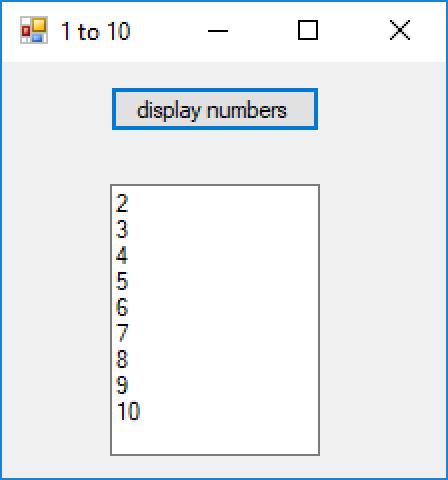
\includegraphics[width=5cm]{repetition_1to10_screen}
			\caption{Display of the numbers 1 to 10.}
			\label{fig:repetition_1to10_screen}
		\end{figure}


	\section{\keyword{For}}
		We begin by using a loop to display the integers 1 to 10 (\Vref{fig:repetition_1to10_screen}) in a multiline text box.
		\begin{lstlisting}
Private Sub Button1_Click(sender As System.Object,
			e As System.EventArgs)
			Handles Button1.Click
	Dim number As Integer
	Textbox1.Clear()
	For number = 1 To 10
		Textbox1.AppendText(CStr(number) & NewLine)
	Next
End Sub
		\end{lstlisting}
		The word \keyword{For} signifies that a repetition is required. The statements enclosed between \keyword{For} and \keyword{Next} are repeated; this is called the \emph{body} of the loop. The repetition starts with the value of \keyword{number} equal to 1, then 2, etc., up to and including \keyword{number} equal to 10. 

		The indentation of the statements within the loop (displayed automatically by the VB development environment) assists us in seeing the structure of the loop.
		
		The text box is initially emptied using the method \keyword{Clear}. Each time the loop repeats, a number is added to the text box using the method \keyword{AppendText}.
		
		This program uses the \keyword{NewLine} property from the VB library. There is also a similar \keyword{Tab} property. To use these, you need an \keyword{Imports} statement like this at the head of the program:
		\begin{lstlisting}
Imports Microsoft.VisualBasic.ControlChars
		\end{lstlisting}
		You will see that this text box allows multiple lines of text to be displayed. In order to accomplish this the \ui{Multiline} property of the text box must be set to \ui{True}.

		A good way to understand how loops work is to use the debugger to follow the execution of this loop. Instead of clicking on the start button, select \ui{Step Into} from the \ui{Debug} menu or alternatively hit the corresponding shortcut key. Repeat to single step through the program. Place the cursor over the text \keyword{number} within the program and watch its value change as the loop proceeds.
		
		This example of a \keyword{For} loop is typical because \keyword{For} loops are normally used when the number of repetitions is known in advance. In the above case we know how many numbers are to be displayed.

		
		This program displays the value of the variable \keyword{number} controlling the loop. Although it is fine to use the value of the variable in this way, it is highly dangerous (and not recommended) to change the value.

		\begin{stqb}
			\begin{STQ}
				\item	What does this program fragment do?
					\begin{lstlisting}
Dim number As Integer
For number = 0 to 5
	TextBox1.AppendText(CStr(number * number) & NewLine))
Next
					\end{lstlisting}
			\end{STQ}
		\end{stqb}
		The next program adds up (calculates the sum of) the numbers 1 to 100. When a button is clicked, the following method calculates and displays the result in a text box.
		\begin{lstlisting}
Private Sub Button1_Click(sender As Object,
	e As System.EventArgs)
	Handles Button1.Click
	Dim number As Integer
	Dim sum As Integer
	sum = 0
	For number = 1 To 100
		sum = sum + number
	Next
	Textbox1.Text = "The sum is " & CStr(sum)
End Sub
		\end{lstlisting}
		This program makes use of a common programming technique - a running total. The value of the variable \keyword{sum} is initially equal to zero. Each time the loop is repeated, the value of \keyword{number} is added to the value of \keyword{sum} and the result placed back in \keyword{sum}.

		The next program uses a \keyword{For} loop to display a row of boxes. The number of boxes is determined by the value selected on a track bar. Whenever the pointer is changed, an event is created and the program displays the matching number of boxes. To do this, we will need a counter. The counter, initially equal to 1, is incremented by one each time a single box is output. We need to repeat the addition of a box until the counter reaches the desired total using a \keyword{For} loop as follows:
		\begin{lstlisting}
Private Sub TrackBar1_Scroll(sender As System.Object,
	e As System.EventArgs)
	Handles TrackBar1.Scroll
	Dim x, numberOfBoxes, counter As Integer
	Dim paper As Graphics
	Dim myPen As Pen = New Pen(Color.Black)
	numberOfBoxes = TrackBar1.Value
	paper = PictureBox1.CreateGraphics()
	paper.Clear(Color.White)	
	x = 10
	For counter = 1 To numberOfBoxes
		paper.DrawRectangle(myPen, x, 10, 10, 10)
		x = x + 15
	Next
End Sub
		\end{lstlisting}
		The output from this piece of program is shown in \Vref{fig:repetition_boxes_screen}.
		
		This program will draw as many boxes as we like. Imagine how many instructions we would have to write in order to display 100 boxes - if we were not able to use a \keyword{For} statement.
		
		\begin{figure}[bth]
			\centering
			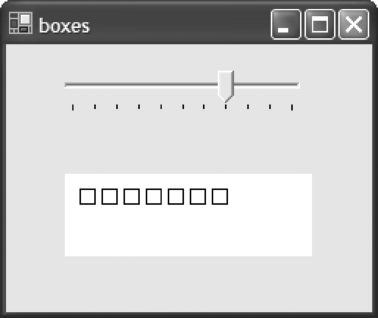
\includegraphics[width=5cm]{repetition_boxes_screen}
			\caption{Screen showing the display of boxes using \keyword{For}.}
			\label{fig:repetition_boxes_screen}
		\end{figure}

		\begin{figure}[th]
			\centering
			\begin{tikzpicture}[node distance=0.8cm,scale=0.8,transform shape]
				\node (start) [startstop] {Begin};
				\node (input) [io, below =of start,align=center] {variable\\=initial value};
				\node (loopstart) [loopstart, below = of input,align=center] {variable\\<= limit ?};
				\node (proc1) [process, align=center, below= of loopstart] {body\\of loop};
				\node (increment) [process, align=center, below= of proc1] {increment\\variable};
				\node (loopstop) [loopstop, below = of increment,align=center] {};
				\node (stop) [startstop, below = of loopstop] {End};
	
				\draw [arrow] (start) -- (input);
				\draw [arrow] (input) -- (loopstart);
				\draw [arrow] (loopstart) -- node[anchor = west,midway] {[variable <= limit]}(proc1);
				\draw [arrow] (proc1) -- (increment);
				\draw [arrow] (increment) -- (loopstop);
				\draw [arrow] (loopstop) -- node[anchor=west,midway] {[variable > limit]} (stop);
			\end{tikzpicture}
			\caption{Flowchart for a \keyword{For} loop.}
			\label{fig:repetition_for_loop}
	 	\end{figure}


		One way to visualize a \keyword{For} loop is using an activity diagram, as shown in \Vref{fig:repetition_for_loop}. The computer normally obeys instructions in sequence from top to bottom as shown by the arrows. A \keyword{For} loop means that the variable is tested before the loop is executed and again before any repetition of the loop. If the value is less than or equal to the final value the loop is executed. When, finally, the value of the variable exceeds the final value, the body of the loop ceases to be executed and the repetition ends.

		\begin{stqb}*
			\begin{STQ}
			\item	\name{Prison bars} Write a program to draw five vertical parallel lines.
			\item	\name{Chessboard} Write a program to draw a chessboard with 9 vertical lines, 10 pixels apart, and 9 horizontal lines, 10 pixels apart.
			\item	\name{Squaring numbers} Write a program to display the numbers 1 to 5 and their squares.
			\end{STQ}
		\end{stqb}


	\section{\keyword{While}}
		The \keyword{While} loop is more flexible than the \keyword{For} loop, but with power comes responsibility.
		
		We have seen how to use loops to repeat something when we knew in advance how many repetitions were needed. But in some situations, we don't know how many repetitions will be needed. As an example illustrating how to use \keyword{While}, we use an old fable about a ruler of India. In the fable someone is asked what he wants as a reward for inventing the game of chess. The response is that he would like as many grains of rice as you would get if you put one on the first square of a chess board, two on the second, four on the third, and so on, doubling the amount on the previous square. Let us write a program to find out how many squares would be needed to get 100 grains of rice. The screen looks like \Vref{fig:repetition_rice_screen}.

		\begin{figure}[bth]
			\centering
			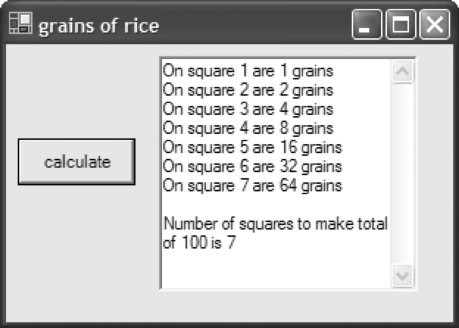
\includegraphics[width=5cm]{repetition_rice_screen}
			\caption{Screen for the grains of rice program.}
			\label{fig:repetition_rice_screen}
		\end{figure}


		We need a loop, but in this situation the significant feature is that we don't know in advance how many repetitions will be needed - this is what we want to find out. Initially the number of grains is 1 and the number of squares is 1. Each time we move to a new square, we add one to the square number and double the number of grains on the new square. We calculate the total amount of rice using a running total, initially equal to zero. We use a multiline text box, set as a property of the text box when the form is designed. We also use a vertical scroll bar with the text box because we do not know in advance how much output will be created by the program. The code is:
		\begin{lstlisting}
Private Sub Button1_Click(sender As Object,
			e As System.EventArgs)	
			Handles Button1.Click
	Dim square, rice, total As Integer
	square = 1
	rice = 1
	total = 1
	DisplayCounts(square, rice)		
	While total < 100
		square = square + 1
		rice = rice * 2
		DisplayCounts(square, rice)
		total = total + rice
	End While
	TextBox1.AppendText(Newline &
			"Number of squares to make total of 100 is " & 
			 square)
End Sub
Private Sub DisplayCounts(square As Integer,
				rice As Integer)
	TextBox1.AppendText("On square " & square &
				" are " & rice & " grains" & NewLine)
End Sub
		\end{lstlisting}
		The \keyword{While} loop works like this. Initially the value of \keyword{total} is equal to 1. This is less than 100, so the loop is carried out and the output created. Then \keyword{total} is increased by the amount of rice on the new square. This is still less than 100, so the loop is repeated again. This continues until total becomes 100 or more and the loop is over. Initially the text box is empty. Each time the loop repeats, a new line of text is appended to the multiline text box using the method \keyword{AppendText}.
		
		The condition determines whether a \keyword{While} loop is executed or completed as follows:
		\begin{itemize}
	    \item If the condition is true, the body of the loop is executed.
			\item If the condition is false, the loop ends and the statements after the \keyword{End While} are executed.
		\end{itemize}
		\keyword{While} loops tend to have the following components:
		\begin{itemize}
    	\item some initialization before the loop (e.g. \keyword{total}  = 1);
	    \item a condition controlling the repetition (e.g. \keyword{total}  < 100);
  	  \item something inside the loop that affects the condition (e.g. \keyword{total = total + rice} ).
		\end{itemize}
		The above program fragment used the less than (<) operator. This is one of a number of available comparison operators, which are the same as those used in \keyword{If} statements. Here, again, is the complete list of the comparison operators:

		\begin{center}
			\begin{tabular}{ll}
				\toprule Symbol &	Means \\ \midrule
				> & greater than\\
				< & less than\\
				= & equals\\
				<>& not equal to\\
				<=& less than or equal to\\
				>=& greater than or equal to\\ \bottomrule
			\end{tabular}
		\end{center}
		One way to visualize how a \keyword{While} statement works is to study an activity diagram, as shown in \Vref{fig:repetition_while_loop}. Notice that, as in the \keyword{For} statement, the test on the condition is made at the start of the loop.

		\begin{figure}[th]
			\centering
			\begin{tikzpicture}[node distance=0.8cm,scale=0.8,transform shape]
				\node (start) [startstop] {Begin};
				\node (input) [io, below =of start,align=center] {variable\\=initial value};
				\node (loopstart) [loopstart, below = of input,align=center] {variable\\<= limit ?};
				\node (proc1) [process, align=center, below= of loopstart] {body\\of loop};
				\node (increment) [process, align=center, below= of proc1] {increment\\variable};
				\node (loopstop) [loopstop, below = of increment,align=center] {};
				\node (stop) [startstop, below = of loopstop] {End};
	
				\draw [arrow] (start) -- (input);
				\draw [arrow] (input) -- (loopstart);
				\draw [arrow] (loopstart) -- node[anchor = west,midway] {[variable <= limit]}(proc1);
				\draw [arrow] (proc1) -- (increment);
				\draw [arrow] (increment) -- (loopstop);
				\draw [arrow] (loopstop) -- node[anchor=west,midway] {[variable > limit]} (stop);
			\end{tikzpicture}
			\caption{Flowchart for a \keyword{While} statement.}
			\label{fig:repetition_while_loop}
	 	\end{figure}


		It is wise to exercise great care when you write a \keyword{While} loop to make sure that the counting is done properly. A common error is to make the loop repeat one too many times or one too few times. This is sometimes known as an 'off by one' error. Sometimes a loop is written so as to start with a count of 0 and the test is to see whether it is less than the number required, as follows:
		\begin{lstlisting}
count = 0
While count < numberRequired
	' loop
	count = count + 1
End While
		\end{lstlisting}
		Alternatively the loop is written to start with a count of 1 and the test is to see whether it is less than or equal to the number required, as follows:
		\begin{lstlisting}
count = 1
While count <= numberRequired
	' loop
	count = count + 1
End While
		\end{lstlisting}
		Both of these styles are used in this book.


	\section{\keyword{And}, \keyword{Or}, \keyword{Not}}
	On occasions, the condition that controls a loop is more complex and we need the \keyword{And}, \keyword{Or} and \keyword{Not} logical operators. You would use these in everyday life if you wanted to say 'I'm going for a walk until it starts raining or it is 5 o'clock.' (We've already met these operators in \Cref{ch:selection} on decisions using the \keyword{If} statement).
		
		If we wanted to describe how long we are going walking for using a \keyword{While} statement, we would say 'While it is not raining and it is not 5 o'clock, I am going walking.' Notice that each of the two conditions (raining, 5 o'clock) is preceded by a 'not' and that the two conditions are linked by an 'and'. This is what tends to happen when you write a loop with a \keyword{While} statement - and you have to be very careful to write the condition very clearly.
		
		We will revisit the grains of rice program. Suppose we want to add up the number of grains as before, but this time we want to stop either when we have got to 64 squares (the number of squares on a chessboard) or when the total is 10 000 grains. So we want the loop to continue while the total is less than 10 000 and the number of squares is less than 64. The program is:
		\begin{lstlisting}
Private Sub Button1_Click(sender As Object,
			e As System.EventArgs)
	Dim square, rice, total As Integer
	square = 1
	rice = 1
	total = 1
	DisplayCounts(square, rice)
	While total < 10000 And square < 64
		square = square + 1
		rice = rice * 2
		total = total + rice
		DisplayCounts(square, rice)
	End While
	TextBox1.AppendText(Newline & "Total is " & total)
	TextBox1.AppendText(NewLine & "on " & square & " squares")
End Sub
Private Sub DisplayCounts(square As Integer,
			rice As Integer)
	TextBox1.AppendText("On square " & square &
			" are " & rice & " grains" & NewLine)
End Sub
		\end{lstlisting}


		\begin{stqb}
			\begin{STQ}
			\item What is displayed when the following code is executed? Is it n = 0 and m = 5 or is it n = 0 and m = −5?
				\begin{lstlisting}
Dim n, m As Integer
n = 10
m = 5
While (n > 0) Or (m > 0)
	n = n - 1
	m = m - 1
End While
MessageBox.Show("n = " & CStr(n) & " m = " & CStr(m))	
				\end{lstlisting}
			\end{STQ}
		\end{stqb}


	\section{\keyword{Do}…\keyword{Loop}}
		If you use \keyword{While}, the test is always carried out at the beginning of the repetition. The \keyword{Do} loop comes in four varieties and in two of the varieties the test is carried out at the end of the loop. You also have the choice of making the test using either \keyword{While} or \keyword{Until}. The best choice is determined by the particular programming situation. We illustrate the different varieties of \keyword{Do} loop by writing pieces of program to display the numbers 0 to 9 in a text box using all the available loop structures.
		
		Using \keyword{For}:
		\begin{lstlisting}
Dim count As Integer
TextBox1.Clear()
For count = 0 To 9
	TextBox1.AppendText(CStr(count))
Next
		\end{lstlisting}
		Using \keyword{While}:
		\begin{lstlisting}
Dim count As Integer
TextBox1.Clear()
count = 0
While count <= 9
	TextBox1.AppendText(CStr(count))
	count = count + 1
End While
		\end{lstlisting}
		Using \keyword{Do} with the test at the start of the loop:
		\begin{lstlisting}
Dim count As Integer
TextBox1.Clear()
count = 0
Do While count <= 9
	TextBox1.AppendText(CStr(count))
	count = count + 1
Loop
		\end{lstlisting}
		Using \keyword{Do} with a different test at the start of the loop:
		\begin{lstlisting}
Dim count As Integer
TextBox1.Clear()
count = 0
Do Until count = 10
	TextBox1.AppendText(CStr(count))
	count = count + 1
Loop
		\end{lstlisting}
		Using \keyword{Do} with the test at the end of the loop:
		\begin{lstlisting}
Dim count As Integer
TextBox1.Clear()
count = 0
Do
	TextBox1.AppendText(CStr(count))
	count = count + 1
Loop While count < 10
		\end{lstlisting}
		Using \keyword{Do} with a different test at the end of the loop:
		\begin{lstlisting}
Dim count As Integer
TextBox1.Clear()
count = 0
Do
	TextBox1.AppendText(CStr(count))
	count = count + 1
Loop Until count = 10
		\end{lstlisting}
		You can see that the choices provided by a \keyword{Do} loop are:
		\begin{itemize}
	    \item testing at either the start or the end of the repetition;
  	  \item testing using either \keyword{While} or \keyword{Until}.
		\end{itemize}


	\section{Nested loops}
		A nested loop is a loop within a loop. Suppose, for example, we want to display the output shown in \Vref{fig:repetition_apartment_screen}, which is a crudely drawn block of apartments. Suppose that there are four floors, each with five apartments, shown as rectangles. The loop that draws an individual floor has this structure:
		\begin{lstlisting}
For apartment = 1 To 5
	' code to draw one apartment
Next
		\end{lstlisting}
		and the loop that draws a number of floors has this structure:
		\begin{lstlisting}
For floor = 1 To 3
	' code to draw one floor
Next
		\end{lstlisting}

		\begin{figure}[bth]
			\centering
			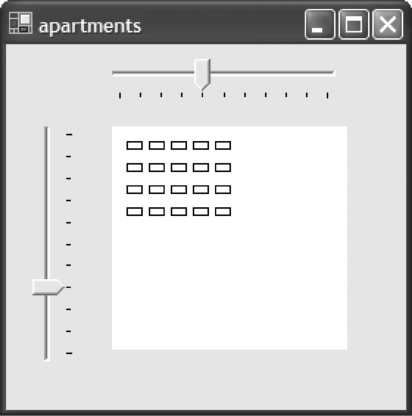
\includegraphics[width=5cm]{repetition_apartment_screen}
			\caption{Display of apartment block.}
			\label{fig:repetition_apartment_screen}
		\end{figure}

		What we need is to enclose the first loop within the second loop so that the loops are nested. We make the number of apartments per floor and the number of floors both set by track bars. Whenever either track bar is changed, an event is caused and we will call this method:
		\begin{lstlisting}
Private Sub DrawFlats(floors As Integer,
				flats As Integer)
	Dim x, y As Integer
	Dim floor, flat As Integer
	Dim paper As Graphics
	paper = PictureBox1.CreateGraphics()
	paper.Clear(Color.White)
	Dim myPen As Pen = New Pen(Color.Black)
	y = 10
	For floor = 0 To floors
		x = 10
		For flat = 0 To flats
			paper.DrawRectangle(myPen, x, y, 10, 5)
			x = x + 15
		Next
		y = y + 15
	Next
End Sub
		\end{lstlisting}
		and you will see that the indentation helps considerably in understanding the program. It is always possible to rewrite nested loops using methods, and this code is sometimes clearer. We explore this further in \Cref{ch:program-style} on style.

		\begin{stqb}
			\begin{STQ}
				\item A music score is written on paper printed with staves. Each stave consists of five horizontal lines across the page, approximately 2 mm (1/10 inch) apart. Each page holds eight of these staves. Write a program to draw a page of musical score.
			\end{STQ}
		\end{stqb}


	\section{Combining control structures}
		In \Cref{ch:selection} we looked at selection using the \keyword{If} statement and in this chapter we have looked at repetition using \keyword{For}, \keyword{While} and \keyword{Do}. Most programs consist of combinations of these control structures. In fact most programs consist of:
		\begin{itemize}
	    \item sequences;
  	  \item loops;
    	\item selections;
	    \item calls of library methods;
  	  \item calls of methods that we, the programmer, write.
		\end{itemize}
		We will now look at an example program where both repetition and selection are used. In this program a ball bounces around the screen, leaving a trace as shown in \Vref{fig:repetition_bouncing_screen}. Its position at any time is specified by its $x$- and $y$-coordinates. Initially it starts at the top left-hand corner of the window. It moves in increments of 7 pixels in the $x$ direction, and 2 in the $y$ direction, and leaves a series of images as it moves. The library method \keyword{DrawEllipse} is used to draw the ball, with diameter 10 pixels. When the ball strikes any of the four walls, its direction is reversed. The ball appears to bounce randomly around the picture box, because of the values chosen for the increments.
		
		\begin{figure}[bth]
			\centering
			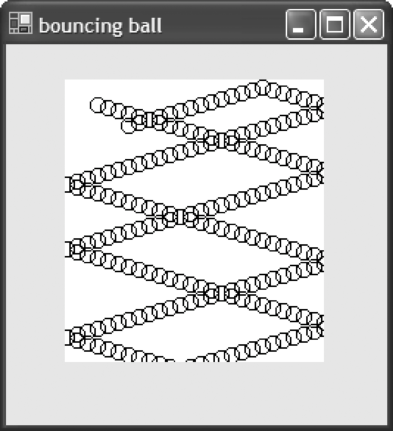
\includegraphics[width=5cm]{repetition_bouncing_screen}
			\caption{The bouncing ball.}
			\label{fig:repetition_bouncing_screen}
		\end{figure}

		
		A \keyword{For} loop causes the ball to move through 200 repetitions. If statements check whether the boundary has been encountered.
		\begin{lstlisting}
Private Sub PictureBox1_Click(sender As Object,
		e As System.EventArgs)
		Handles PictureBox1.Click
	Dim x, y, diameter, count As Integer
	Dim xChange As Integer = 7
	Dim yChange As Integer = 2
	x = 10
	y = 10
	diameter = 10
	For count = 1 To 200
		MoveBall(x, y, xChange, yChange)
		DrawBall(x, y, diameter)
	Next
End Sub
Private Sub MoveBall(ByRef x As Integer,
		ByRef y As Integer,
		ByRef xChange As Integer,
		ByRef yChange As Integer)
	If x <= 0 Then
		xChange = -xChange
	End If
	If x >= PictureBox1.Width Then
		xChange = -xChange
	End If
	If y <= 0 Then
		yChange = -yChange
	End If
	If y >= PictureBox1.Height Then
		yChange = -yChange
	End If
	x = x + xChange
	y = y + yChange
End Sub
Private Sub DrawBall(x As Integer,
			y As Integer,
			diameter As Integer)
	Dim paper As Graphics
	paper = PictureBox1.CreateGraphics()			
	Dim myPen As Pen = New Pen(Color.Black)
	paper.DrawEllipse(myPen, x, y, diameter, diameter)
End Sub
		\end{lstlisting}
		This is a typical example of a program in which loops and selection are used together.


	\section{Programming principles}
		There are three varieties of looping statement - \keyword{For}, \keyword{While} and \keyword{Do}. So which one do you choose to use? The guidelines are:
		\begin{itemize}
	    \item The \keyword{For} loop is used when the number of repetitions is known in advance. A \keyword{For} loop repeats zero or more times.
	    \item The \keyword{While} loop is generally used when the number of repetitions that will be needed is not known in advance. A \keyword{While} loop can be used for zero or more repetitions.
  	  \item The \keyword{Do} loop is used as a style alternative, or when the test for the end of the repetition needs to be made at the end of the loop.
		\end{itemize}
		Thus the most widely applicable facility is the \keyword{While} loop, but it isn't necessarily the most appropriate choice in all circumstances. If \keyword{For} and \keyword{Do} were abolished from VB, we would manage without them by using \keyword{While}, but on the right occasion they are simply the best thing to use.
		
		Loops come into their own in programs that process collections of data. We will meet various collections later in this book. They include strings, files, arrays and databases.


	\section{Programming pitfalls}
		\begin{itemize}
  	  \item In \keyword{While} statements, be very careful with the condition. It is a very common error to make a loop finish one repetition too early or else repeat once too many times.
    	\item Be careful with complex conditions in \keyword{While} loops. \keyword{Do} you need \keyword{Or} or do you need \keyword{And}?
	    \item Within a \keyword{For} loop, do not alter the value of the controlling variable.
			\item To use \keyword{Tab} and \keyword{NewLine}, you need an \keyword{Imports} statement like this at the head of the program:
				\begin{lstlisting}
Imports Microsoft.VisualBasic.ControlChars
				\end{lstlisting}
		\end{itemize}


	\section{Grammar spot}
		\begin{itemize}
	    \item The \keyword{For} loop has the structure:
				\begin{lstlisting}
For variable = startValue To endValue
	statement(s)
Next
				\end{lstlisting}
				where variable is an \keyword{Integer} variable, \keyword{startValue} and \keyword{endValue} are \keyword{Integer} values. Notice that all other statements have an End statement to match, but because of a historical legacy VB breaks its grammatical rules with the \keyword{For}.
	    \item The \keyword{While} loop has the structure:
				\begin{lstlisting}
While condition
	statement(s)
End While
				\end{lstlisting}
				where the condition is tested before any repetition of the loop. If it is true, the loop continues. If it is false, the loop ends.
	    \item The \keyword{Do} loop has four alternative structures:
				\begin{lstlisting}
Do While condition
	statement(s)
Loop
Do Until condition
	statement(s)
Loop
Do
	statement(s)
Loop While condition
Do
	statement(s)
Loop Until condition
				\end{lstlisting}
				In the first two varieties, the test is performed before each repetition and in the last two varieties, the test is performed after each repetition.
		\end{itemize}


	\section{New language elements}
	\begin{itemize}
    \item The control structures for repetition:
			\begin{quote}
\keyword{For} and \keyword{Next}

\keyword{While} and \keyword{End While}

\keyword{Do} and \keyword{Loop}
			\end{quote}
	\end{itemize}


	\section{Summary}
		\begin{itemize}
	    \item A repetition in programming is called a loop.
  	  \item There are three ways in VB of instructing the computer to loop - \keyword{For}, \keyword{While} and \keyword{Do}.
    	\item Use \keyword{For} when you know in advance how many repetitions will have to be performed.
	    \item Use \keyword{While} when you do not know in advance how many repetitions will have to be performed.
  	  \item \keyword{Do} is used as an alternative style or when a condition needs to be tested at the end of a loop.
		\end{itemize}


	\section{Exercises}
		\begin{EXE}
			\item	\name{Display} integers Write a program to display the integer numbers 1 to 10 and the cubes of each of their values using a loop.
			\item	\name{Random numbers} Write a program to display 10 random numbers using a loop. Use the library class Random to obtain random numbers in the range 1 to 100. Display the numbers in a text box.
			\item	\name{The milky way} Write a program that draws 100 circles in a picture box at random positions and with random diameters up to 100 pixels.
			\item	\name{Steps} Write a program to draw a set of steps made from bricks, as shown in \Vref{fig:repetition_steps_screen}. Use the library method DrawRectangle to draw each brick.
				\begin{figure}[bth]
					\centering
					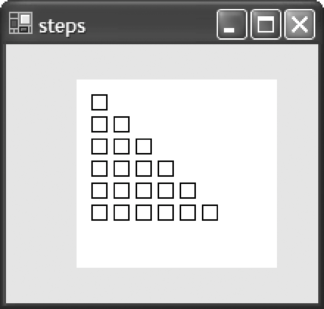
\includegraphics[width=5cm]{repetition_steps_screen}
					\caption{Screen of \name{Steps}.}
					\label{fig:repetition_steps_screen}
				\end{figure}
			\item	\name{Sum of the integers} Write a program that adds up the numbers 0 to 39 using a loop. Check that it has obtained the right answer by using the formula for the sum of the numbers 0 to n:
				\begin{lstlisting}
sum = n × (n + 1)/2
				\end{lstlisting}
			\item	\name{Saw-tooth pattern} Write a program to display a saw-tooth pattern, as shown in \Vref{fig:repetition_sawtooth_screen}, in a text box.
				\begin{figure}[bth]
					\centering
					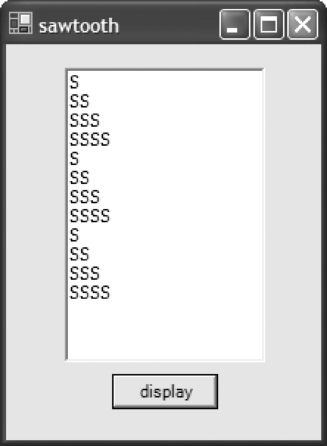
\includegraphics[width=5cm]{repetition_sawtooth_screen}
					\caption{Saw-tooth pattern.}
					\label{fig:repetition_sawtooth_screen}
				\end{figure}
			\item	\name{Multiplication table} Write a program to display a multiplication table, such as young children use. For example, the table for numbers up to 6 is shown in \Vref{fig:repetition_multiplication_screen}.
				The program should be capable of displaying a table of any size, specified by an integer entered into a text box. Use the library \keyword{Tab} property.
				\begin{figure}[bth]
					\centering
					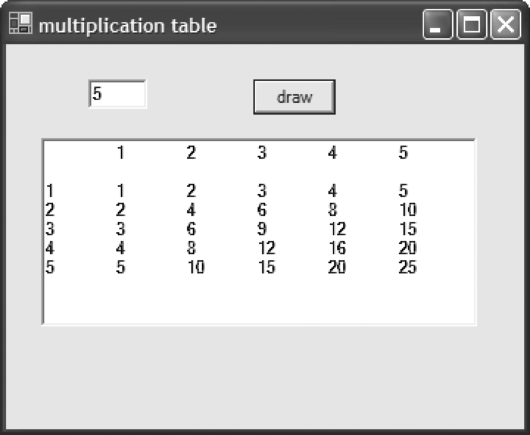
\includegraphics[width=5cm]{repetition_multiplication_screen}
					\caption{Multiplication table.}
					\label{fig:repetition_multiplication_screen}
				\end{figure}
			\item	\name{Fibonacci} The Fibonacci series is the series of numbers:
				\begin{lstlisting}
1  1  2  3  5  8  13...
				\end{lstlisting}
				Each number (except for the first two), is the sum of the previous two numbers. 
				
				The first two numbers are 1 and 1. The series is supposed to govern growth in plants. Write a program to calculate and display the first 20 Fibonacci numbers.
			\item	\name{Sum of series} Write a program to calculate and display the sum of the series:
				\begin{lstlisting}
1 − 1/2 + 1/3 − 1/4 + . . .
				\end{lstlisting}
				until a term is reached that is less than 0.0001.
			\item	\name{Bouncing ball} The bouncing ball program could do with some improvements. First, it doesn't bounce properly when it hits a wall. Alter it so that whenever any part of the ball hits a wall it bounces. Provide a feature to alter the direction that the ball moves in, using text boxes to specify the x and y pixel changes. Provide a feature so that the picture box looks like a pool table with a single pocket right in the middle of the table down which the ball will vanish.
			\item \name{Nursery rhyme} Write a program to display all the verses of a nursery rhyme in a text box with a vertical scrollbar. The first verse is:
				\begin{quote}
					10 green bottles, hanging on a wall,

					10 green bottles, hanging on a wall,

					If 1 green bottle were to accidentally fall

					There'd be 9 green bottles, hanging on the wall.
				\end{quote}
				In successive verses there are reduced numbers of bottles, as they fall off the wall.

		\end{EXE}
		
		\begin{stab}
			\begin{enumChapter}
				\item	It displays the numbers 0 1 4 9 16 25 on separate lines.
				\item	\ \begin{lstlisting}
Dim x, numberOfBars, counter As Integer
Dim paper As Graphics
Dim myPen As Pen = New Pen(Color.Black)
numberOfBars = 5
paper = PictureBox1.CreateGraphics()
paper.Clear(Color.White)
x = 10
For counter = 1 To numberOfBars
	paper.DrawLine(myPen, x, 10, x, 100)	
	x = x + 15
Next
					\end{lstlisting}
				\item \
					\begin{lstlisting}
Dim x, y, counter As Integer
Dim paper As Graphics
Dim myPen As Pen = New Pen(Color.Black)
paper = PictureBox1.CreateGraphics()	
paper.Clear(Color.White)
x = 10
For counter = 1 To 9
	paper.DrawLine(myPen, x, 10, x, 90)
	x = x + 10
Next
y = 10
For counter = 1 To 9
	paper.DrawLine(myPen, 10, y, 90, y)
	y = y + 10
Next
					\end{lstlisting}
				\item \
					\begin{lstlisting}
Dim number As Integer
For number = 1 To 5
	TextBox1.AppendText(CStr(number) &
	CStr(number * number) & NewLine)
Next
					\end{lstlisting}
				\item	n = 0 and m = −5.
				\item \
					\begin{lstlisting}
Dim y, staves, lines As Integer
Dim paper As Graphics
Dim myPen As Pen = New Pen(Color.Black)
paper = PictureBox1.CreateGraphics()
paper.Clear(Color.White)
y = 10
For staves = 1 To 8
	For lines = 1 To 5
		paper.DrawLine(myPen, 10, y, 90, y)
		y = y + 2
	Next
	y = y + 5
Next
					\end{lstlisting}
			\end{enumChapter}
		\end{stab}%
